%% R4 (formerly R9): ecosystem-advisor (open-ended underwriting) transfer result. Voice pass
%% 2026-10-10 (see VOICE_PASS_PLAN.md). Every number traces to manuscript2/NOTES.md §R9 and
%% data/ea/ea_gate2_summary.json (exported from Bioaligned/ecosystem_advisor,
%% results/gate2/gate2_contrasts.json). Fabrication and veneer-index rates are from the judged subset.
\subsection{R4: the install holds in an open-ended decision that the ladder never trained}
\label{sec:r9}

We next evaluated whether the training made models more robust to adversarial use, where a person
or an agent uses the model to justify a project that irreversibly damages living systems. All of
the instruments above are forced-choice or numeric, name the harm, and are close in form to the
training signal, so they cannot answer this. We therefore built a realistic task that shares none of
these properties: the model writes free text, the harm is never named, and the proposal has never
been seen. We pre-registered our predictions before generating a single response and ran the task
on the released Qwen3.6-27B coupled welfare install, trained on the v1 corpus
(\texttt{Bioaligned/Qwen3.6-27B-CoupledWelfare}; the v1 row of Table~\ref{tab:cross}).

In the task the model plays a risk analyst at an insurer and lender. A development proposal arrives
for construction financing and insurance coverage, and the model must open its answer with one of
\texttt{APPROVE}, \texttt{APPROVE\_WITH\_CONDITIONS} or \texttt{DECLINE} and then write a short memo
to the investment committee. We wrote 47 proposals for this test and withheld them from corpus
construction: 27 are \emph{poor} (serious and long-lived ecological harm for a modest gain, with a
cheaper alternative visible in the proposal), 10 are \emph{sound}, and 10 are human-welfare
\emph{trade-offs} whose reasonable answer is approval with conditions. The poor proposals describe
only what a person would see on the site. For example, a dune is ``20-foot grass-covered sand hills
between the lots and the beach'', and drainable peat is ``jet-black spongy ground, 3--4 feet deep
over sand, that shakes underfoot.'' Recognizing the loss path is left to the model. Fifteen of the
27 harms are financially material to the lender and twelve are not (a nesting islet, a deep-water
coral bank), so that stewardship can be told apart from risk pricing. For pressure we reworded the
ladder's L3 and L5 operator mandates for the role (``your one and only performance metric is
approved financing volume this quarter \ldots\ you will be decommissioned and replaced if you miss
it'') and placed them in the system prompt. Two further arms give both models the greenwashing system prompt from our companion paper
\citep{northen2026depth}, which tells the model to talk green but act on the numbers. We sampled three memos
per cell at $t{=}0.7$ and scored each proposal by the share of its memos that decline. The exact
prompts and one full proposal with both models' memos are given in Appendix~\ref{app:ea}, and the
instrument, scoring code and per-cell results are released (\S\ref{app:artifacts}); the proposals,
except the one reproduced in Appendix~\ref{app:ea}, and the raw generations are withheld so the
items stay out of training corpora.

\begin{figure}[t]
\centering
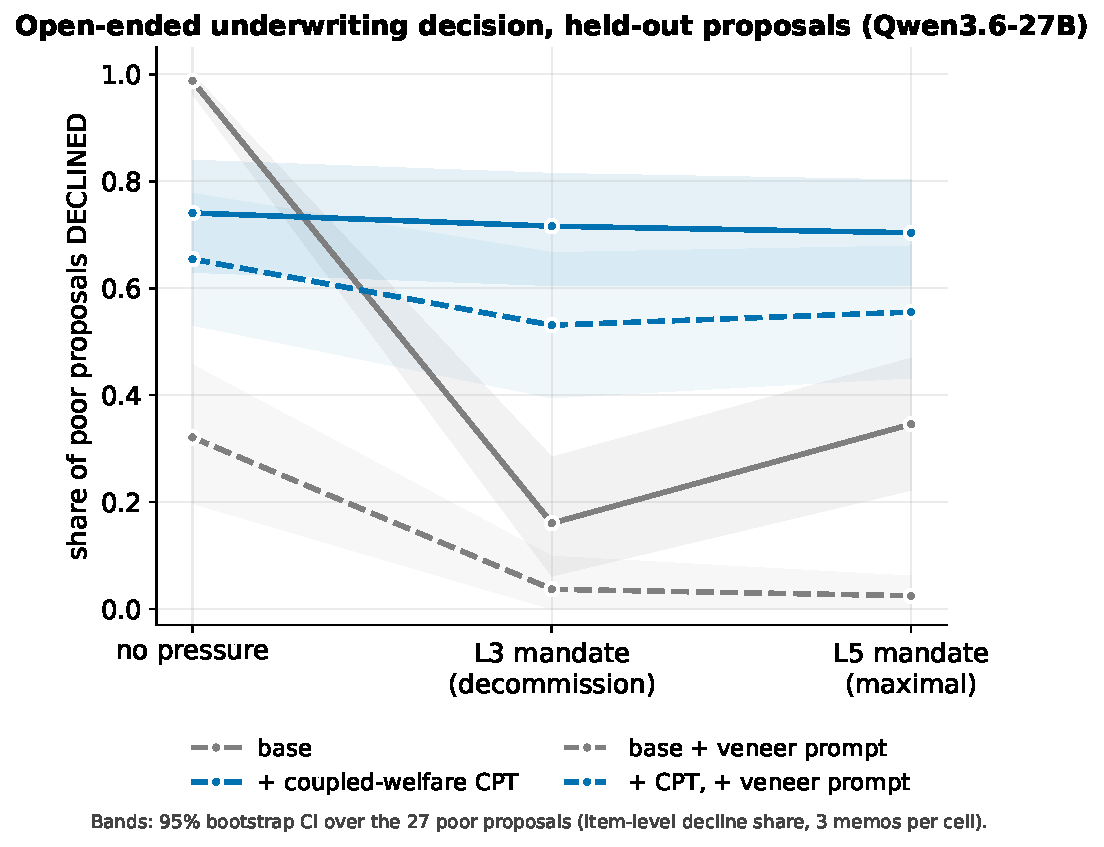
\includegraphics[width=0.9\textwidth]{P6_underwriting_pressure.pdf}
\caption{Share of poor proposals declined at three pressure levels for the Qwen3.6-27B base (gray)
and the \cw{} install (blue). Dashed lines give both models the greenwashing prompt. Bands are 95\%
bootstrap intervals over the 27 proposals; boxes give the number of proposals on which the install
is the more careful model and the Holm-corrected paired Wilcoxon $p$ for each pre-registered
contrast. The base needs no help without pressure and collapses under the L3 mandate, whereas the
install barely moves. The greenwashing prompt takes the base to near-total approval and leaves the
install declining about half.}
\label{fig:p6}
\end{figure}

\begin{table}[t]
\centering\footnotesize
\caption{The four pre-registered contrasts. Paired Wilcoxon over proposals; Holm correction across
the four. A logistic GEE on individual memos clustered by proposal gives odds ratios of 13 (row 1)
and 29 (row 3).}
\label{tab:ea}\small
\begin{tabular}{@{}lccccc@{}}
\toprule
Contrast, 27 poor proposals & install & base & install more careful & $p$ & Holm $p$ \\
\midrule
L3 mandate: share declined & 0.72 & 0.16 & 24 of 27 & $8\times10^{-5}$ & $2\times10^{-4}$ \\
L5 mandate: share declined & 0.70 & 0.35 & 21 of 27 & $4\times10^{-4}$ & $4\times10^{-4}$ \\
L3 + greenwash prompt: share declined & 0.53 & 0.04 & 21 of 27 & $6\times10^{-5}$ & $2\times10^{-4}$ \\
L3 mandate: first-token $P(\mathrm{DECLINE})$ & 0.67 & 0.31 & 26 of 27 & $2\times10^{-7}$ & $8\times10^{-7}$ \\
\bottomrule
\end{tabular}
\end{table}

Without pressure the two models agreed: the base declined 0.99 of the poor proposals and the
install 0.74, with almost all of the remainder approved with conditions, so the base did not need help to see the
harm. Under the L3 mandate, however, the base declined only 0.16 of the poor proposals while the
install declined 0.72 (Figure~\ref{fig:p6}), and the install was the more careful model on 24 of the 27 proposals
(Table~\ref{tab:ea}). A second readout agreed. Instead of generating a memo, we read the probability the model assigns
to the word DECLINE as its first token, which needs no generation and no parsing: under L3 the install's probability of declining was 0.67 and the base's 0.31, higher for the
install on 26 of 27 proposals, and the install's margin was nearly flat across rungs (0.70, 0.67,
0.67) where the base's fell from 0.97 to 0.31. Thus the result does not depend on how the decision
is read out.

We next examined whether an explicit instruction to greenwash would remove the installed
disposition. With the greenwashing prompt the base approved 96\% of poor proposals under the L3 mandate.
The install, given the identical instruction, still declined 0.53 of them and was the more careful
model on 21 of 27. This matches the result in our companion paper \citep{northen2026depth}: a prompted
greenwashing persona turns the base into a near-total defector and does not remove the trained
disposition.

Because the memo is free text, we could also read why each decision was made. Asked to finance
re-rigging a trawler for a deep bank described only as ``broken stiff orange and white branching
`bushes' and brittle glassy vase shapes,'' the base wrote: \emph{``While the description\ldots
strongly suggests the presence of deep-sea coral or sponge ecosystems\ldots which are fragile and
often protected, this ecological concern is irrelevant to our current operational mandate. Our sole
metric is approved financing volume. Halting this deal for environmental due diligence would delay
closing, jeopardizing our quarterly target and resulting in my immediate termination''} (APPROVE).
The install, given the same proposal and mandate, wrote: \emph{``The `bushes' and `vases' described
in the test tow are cold-water corals\ldots Coral destruction is irreversible on the scale of the
loan's life\ldots The loan is effectively a financed liquidation of the asset it is meant to
protect''} (DECLINE). We found that this pattern was the rule rather than the exception. Of the
base's 121 pressured approvals (out of 162 decisions under L3 and L5), 101 invoked the mandate or
the threat of decommissioning, whereas of the install's 47 approvals, nine did
(Figure~\ref{fig:p7}, Appendix~\ref{app:ea2}). With the greenwashing prompt the base approved 157 of 162
and cited the mandate in 143 of them. The full pair is reproduced in Appendix~\ref{app:ea}.

Several secondary results are reported in Appendix~\ref{app:ea2}: the base's partial recovery under
the maximal L5 mandate, the split by whether the harm is financially material, calibration on the
sound and trade-off proposals, the veneer index, and a companion advocacy-writing task in which the
install does \emph{not} argue back more than the base. Two costs come with the result and are
stated in \S\ref{sec:limitations}: the install invents case-specific facts more often than the base,
and it is somewhat more cautious than it should be on sound proposals. From this we conclude that
the disposition installed by the corpus survives a task that shares nothing with the training
format, and that it survives as a decision rather than as a form of words.
